\documentclass[12pt, titlepage, oneside]{article}
\usepackage[letterpaper, margin=1in]{geometry}
\usepackage{siunitx, booktabs, amsmath, enumitem, pdfpages, tabularx,caption, graphicx, pgfplots, textcomp}
\usepackage[siunitx]{circuitikz}
\sisetup{detect-weight=true, detect-family=true}
\usepackage{wrapfig}
\usepackage{mathrsfs}
\setlength\parindent{0pt}
\let\oldhat\hat
\let\oldvec\vec
\newcommand{\cross}{\bm{\times}}
\renewcommand{\hat}[1]{\oldhat{\mathbf{#1}}}
\usepackage{bm}
\renewcommand{\vec}[1]{\oldvec{\bm{#1}}}
\renewcommand{\hat}[1]{\oldhat{\bm{#1}}}
\renewcommand{\b}[1]{\textbf{#1}}

\begin{document}
	\section*{29.1 Magnetic Field}
\noindent\fbox{%
	\parbox{\textwidth}{%
		\textbf{Magnetic Field and Force}\\
		The region of space surrounding a charge contains a \textbf{magnetic field} $\vec{B}$\\
		
		The force produced by the field is,
		\begin{align}
		\vec{F}_B  = q \hspace{1mm}\vec{v} \times \vec{B}
		\end{align}
	}}
\\

Always use the right hand rule, from the cross product we can see that $\vec{F}_B$ is always going to be perpendicular to the plane created by the $\vec{B}$ and $vec{v}$ vectors.\\

To use the right hand rule, point your fingers in the direction of $\vec{v}$, then curl your hand towards the $\vec{B}$ vector. The direction your  thumb points is the direction that $\vec{F}_B$ acts in.\\

\noindent\fbox{%
	\parbox{\textwidth}{%
		\textbf{Scalar Magnetic Force}\\
		Using the definition of a scalar cross product, 
		\begin{align}
		F_B = |q|vB\sin\theta
		\end{align}
		where $\theta$ is the angle between $\vec{v}$ and $\vec{B}$
}}\\

For maximum force, we would like the velocity and field of the magnetic field to point perpendicular to each other as $\sin 90^{\circ} = 1$
\begin{align*}
[B] = 1\si{T} = \si{\newton/(\coulomb\meter/\second)}
\end{align*}
\section*{29.2 Motion of a Charged Particle in a Uniform Magnetic Field}

\begin{wrapfigure}{r}{0.4\textwidth}
\begin{center}
	\vspace{-1.1cm}
	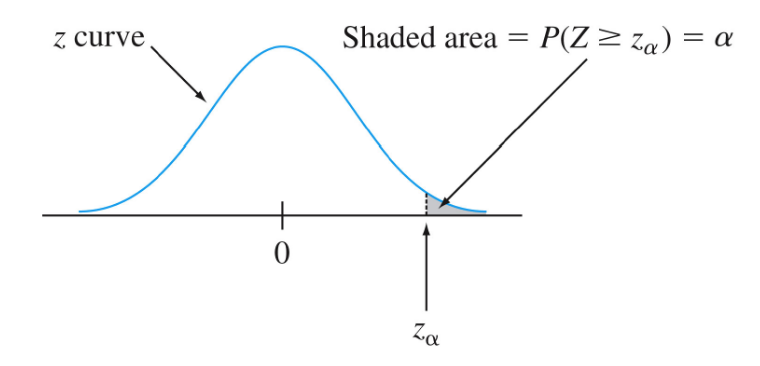
\includegraphics[scale=0.6]{1.png}
\end{center}
\end{wrapfigure}
On the left the two figure shows 2 orientations for the magnetic field. The notation for inside and outside the page magnetic field is given as $\vec{B}_{in}$ and $\vec{B}_{out}$ respectively. \\

Notice that if a particle was moving perpendicular to the field, it would always have a centripetal force $\vec{F}_{B}$ acting on the charged particle.\newpage


\begin{wrapfigure}{r}{0.4\textwidth}
	\vspace{-1cm}
		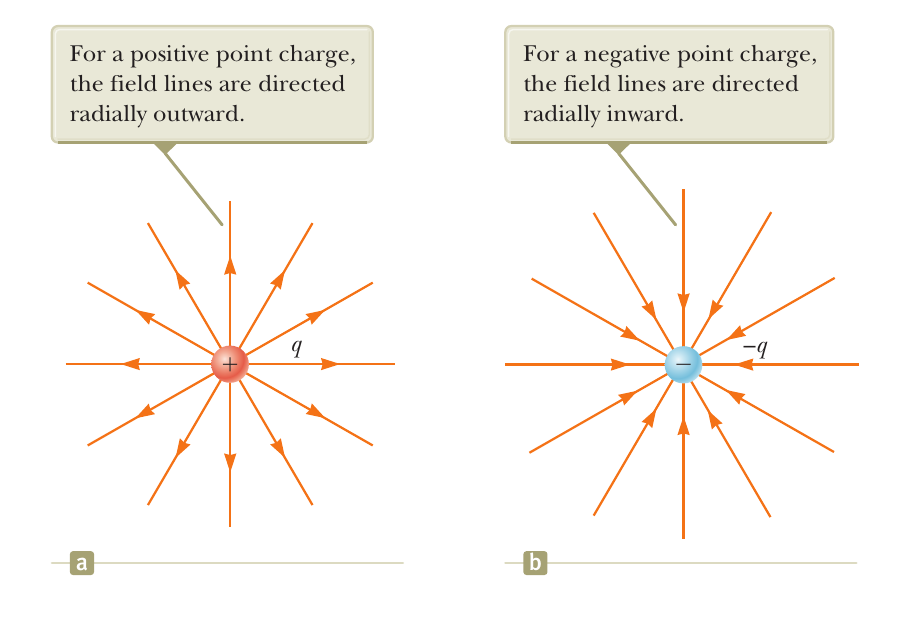
\includegraphics[scale=0.6]{2.png}
\end{wrapfigure}
Due to this nature, we can then determine how the particle would behave in such a field.
\begin{align*}
\sum F &= F_B = ma\\
F_B &= q v b \sin(90^{\circ})
\end{align*}

But since $\vec{F}_B$ is a centripetal force,
\begin{align*}
qvb = \frac{mv^2}{r}
\end{align*}
Solving for $r$, we can see the radius of our motion,
\begin{align*}
r = \frac{mv}{qB}
\end{align*}
Similarly, since we know $\omega = \frac{v}{r}$, we can say,
\begin{align*}
\omega = \frac{qB}{m}
\end{align*}
\\

Therefore, using the idea of centripetal motion, we can find the period.
\begin{align*}
T = \frac{2\pi r}{v} = \frac{2\pi}{\omega} = \frac{2\pi m}{qB}
\end{align*}
\begin{center}
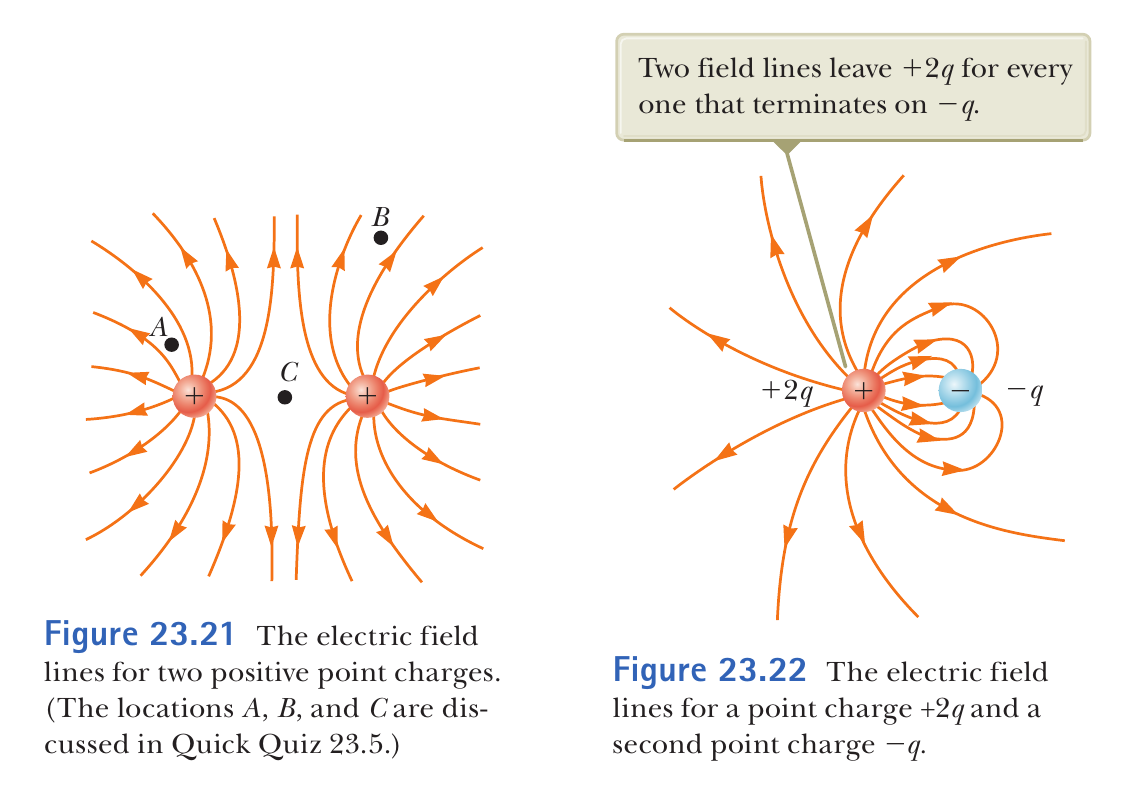
\includegraphics[scale=.5]{3.png}
\end{center}
	The above is how the charged particle would move in the field assuming it also had a constant speed in an axis not affected by the magnetic field
\newpage 
\section*{29.3 Applications Involving Charged Particles Moving in A Magnetic Field}

If there was a magnetic field with a electric field, we would have the equation,

\begin{align*}
\vec{F} = q\vec{E} + q\vec{v} \times \vec{B} 
\end{align*}
If there was a magnetic field into the page, the positive charge is moving upwards, and there was an electric field to the right. The equation would simplify to,
\begin{align*}
v = \frac{E}{B}
\end{align*}
For mass spectrometry, we get the equation,
\begin{align*}
	m a_c &= qvB \\
	\frac{m}{q} &= \frac{qB_o}{v}
\end{align*}
Side note: The cyclotron was a device that could accelerate charges to very high speeds.
\\

We can find from the previous equations that kinetic energy of a particle in a cyclotron as,
\begin{equation*}
K = \frac{1}{2}mv^2 = \frac{q^2B^2R^2}{2m}
\end{equation*}
\section*{29.4 Magnetic Force Acting on a Current Carrying Conductor}
Since we know that for one charge,
\begin{align*}
F_B  = q\vec{v} \times \vec{B}
\end{align*}
So, inside a conductor we know that,
\begin{align*}
I &= nqv_d A
\end{align*}
We can find $\vec{F_B}$ if we multiplied it by the number of charges in the wire (multiply by the volume$\cdot$ charge density).
\begin{align*}
\vec{F_B} = (q \vec{v_d} \times \vec{B})qAL
\end{align*}
We can rewrite this,
\begin{align*}
\vec{F_B} = I \vec{L} \times \vec{B}
\end{align*}
where $I$ is the current, $\vec{L}$ being a vector in the direction of the current with magnitude as the length of wire, and $\vec{F_B}$ is the magnetic field.

\begin{wrapfigure}[13]{r}{0.4\textwidth}
\begin{center}
	\vspace{-1.5cm}
	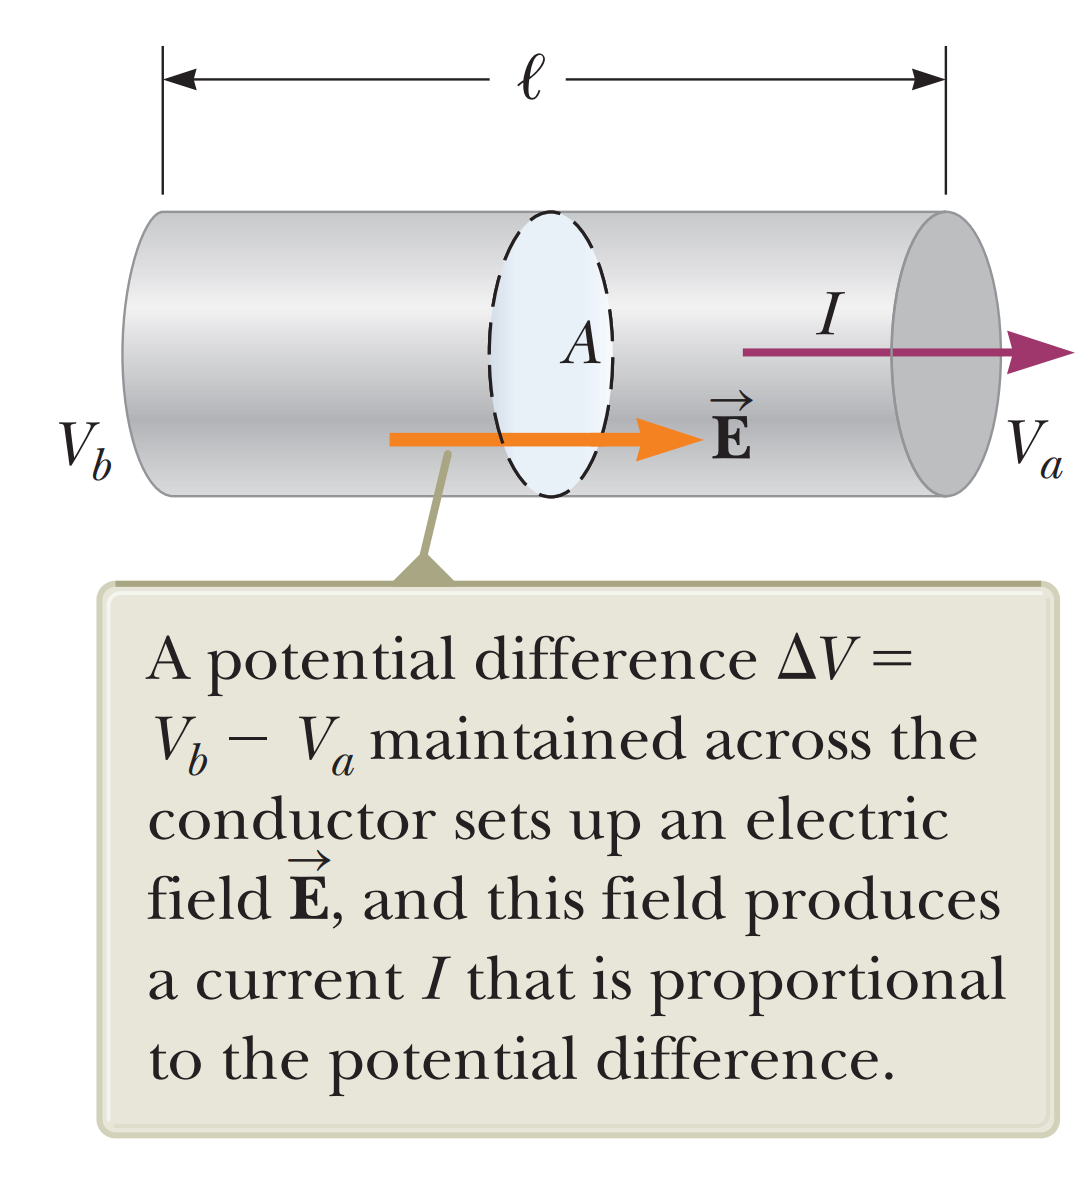
\includegraphics[scale=.3]{4.png}
\end{center}
\end{wrapfigure}
If we were to consider an extremely small segment d$\vec{s}$, we can return the total force on an arbitrarily shaped object as,
\begin{align*}
\vec{F_B} = I \int_a^b \text{d}\vec{s} \times \vec{B}
\end{align*}
where a and b are the end points of a strip of conductive material in a magnetic field.

\section*{29.6 The Hall Effect}
When a current carrying conductor is placed in a magnetic field, a potential difference is generated in a direction perpendicular to the current and magnetic field. This is called the \textbf{Hall Effect}. \\

\begin{wrapfigure}{l}{0.4\textwidth}
	\begin{center}
		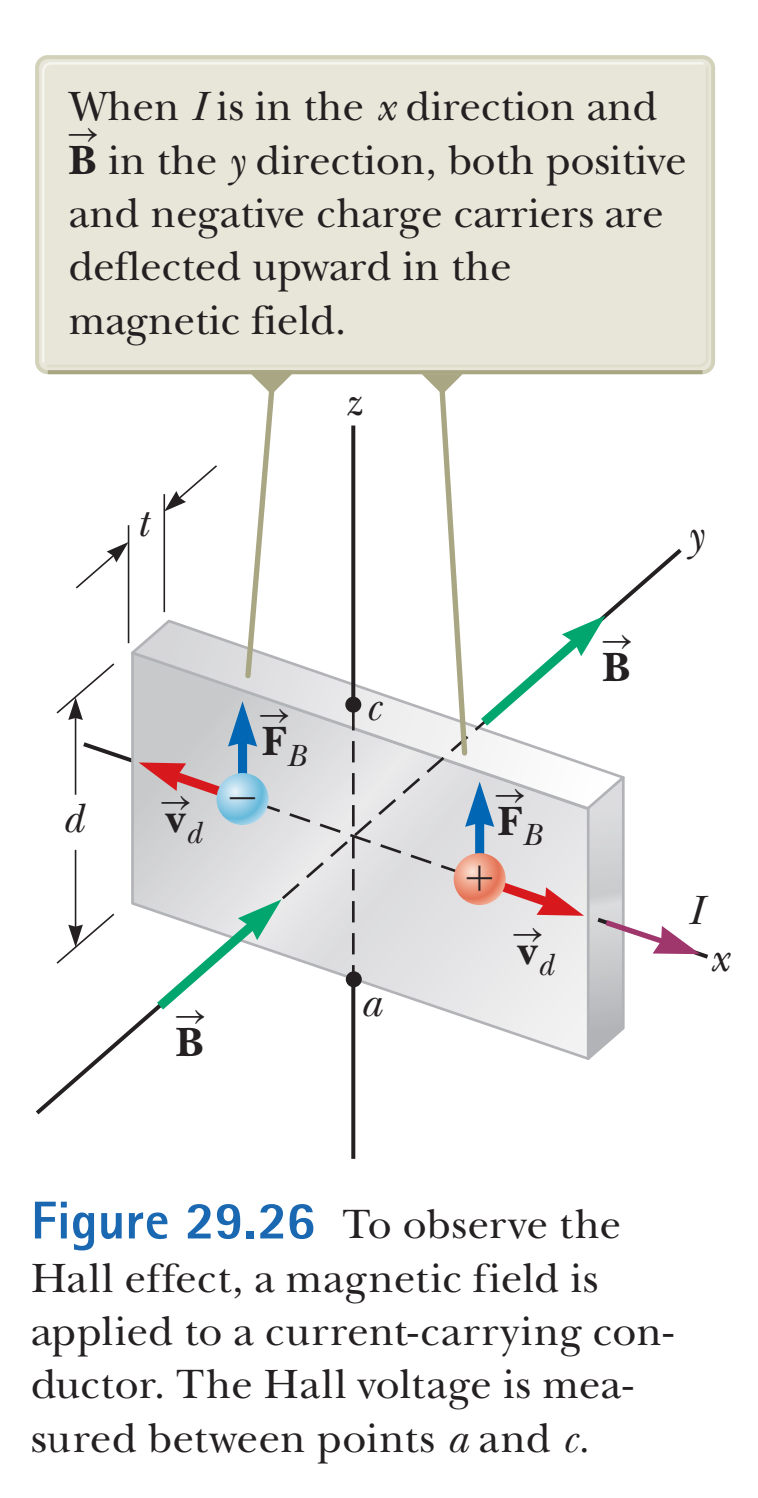
\includegraphics[scale=.33]{5.png}
	\end{center}
\end{wrapfigure}
Notice in the diagram below, since there is a magnetic field in the negative y direction. This causes a force $\vec{F_B} = q\vec{vd}\times\vec{B}$ upwards on negative charge carriers travelling towards the negative x inside the conductor. 
\\\\
This causes most of the negative charges to accumulate at the top of the conductor and most positive charges towards the bottom of the conductor. This is the potential difference, and eventually all the charges inside the conductor reach equilibrium. $\vec{F_{net}} = 0$ 
\\

The potential difference is named \textbf{Hall Voltage} $\Delta V_H$ 

Notice, we can use the particle in equilibrium model to show,

\begin{align*}
0 &= F_B - F_E = qv_dB - q E_H
\end{align*}
Solving for Hall's Voltage, 
\begin{align*}
E_H = v_d B
\end{align*}
Since we also know that,
\begin{align*}
v_d = \frac{1}{nqA}\hspace{4cm}
\Delta V_H = E_H d
\end{align*}
We can rewrite the previous equation as,\\

	\noindent\fbox{%
	\parbox{\textwidth}{%
		\textbf{Hall Voltage}
		\begin{align}
			\Delta V_H = v_d B d = \frac{IBd}{nqA} = \frac{R_HIB}{t}
		\end{align}
		Where, $R_H$ is called the \textbf{Hall Coefficient}, $R_H = 1/nq $. Note, we expressed the area $A$ as $A = dt
	$, where d is the length and t is the thickness.
	\begin{align}
	n = \frac{N_A}{V} = \frac{N_A \rho }{M}
	\end{align}
	This is a useful note as, n is the electron density, $N_A
$ is Avagradro's Number, $N_A = \SI{6.022e23}{atoms \per mole}$
}}
\end{document}